\chapter{Chapter: Threat Modelling}
\label{chap:threat_model}
Threat modelling is an act of security analysis which aids in discovering potential vulnerabilities in an application or a system before they become threats \citep{threat_model_intro}. This exercise is a crucial step in the Software Development Life Cycle (SDLC), as it helps detect the possible flaws in the system, and suitable mitigation can be applied. Similarly, threat modelling will also be conducted for this project, where an authentication server using OIDC protocol is operated in a cloud environment. The approach that this project will apply to threat modelling is based on Shostack's Four Question Framework \citep{shostack}. The questions focus on the project objectives, what could go wrong there, what mitigations could be applied, and whether it can be improved. Using Shostacks questions in conjunction with the OWASP threat modelling process, the application, using OpenID Connect in Cloud, can be analysed \citep{owasp_threat_model}. The objective of threat modelling is to identify as many possible risks present in the Open ID Connect application running on a cloud. Furthermore, the modelling will be cloud agnostic, meaning these identified mitigations can be applied anywhere, irrespective of the cloud provider.


\section{Application Information}
To answer the first question about \textit{what are we working on}, this section will describe the application and the different dependencies that this application contains.
\begin{itemize}
    \item \textbf{Application Name:} Multi-tenant App
    \item \textbf{Application Version:} v1.0
    \item \textbf{Description:} This generic authentication and authorisation application utilises OpenID Connect protocols PKCE flow (See Figure \ref{fig:pkce_flow}) in a public cloud environment. This application will be based on multitenant capability, where the users cannot access each other's resources even though they share the same infrastructure and application. This general API would provide the capabilities mentioned in Table \ref{table:threat_model_entry_points}.
  \end{itemize}

\subsection{Entry Points}
\begin{longtable}{|p{3cm}|p{4cm}|p{4cm}|p{4cm}|}
\caption{Entry Points}
\label{table:threat_model_entry_points}
\hline
\rowcolor{grey!15}
\textbf{Entry Point} & \textbf{Description} & \textbf{Request Parameters} & \textbf{Response Data} \\
\hline
\endfirsthead
\hline
\rowcolor{grey!15}
\textbf{Entry Point} & \textbf{Description} & \textbf{Request Parameters} & \textbf{Response Data} \\
\hline
\endhead
\endfoot
\hline
\endlastfoot

/authorize & Entry point for user authentication.  & 
- client\_id: The client ID of the application \newline 
%- redirect\_uri: URI where the response will be sent \newline
- scope: Scopes for requested authentication (e.g., OpenID, email) \newline 
- response\_type: Indicates the desired authorization flow (e.g., code) & 
- The authorisation code is to be exchanged for tokens. \newline 
- Error in case of invalid request \\
\hline

/token & Entry point for exchanging authorization code for tokens (access token, ID token, refresh token). & 
- grant\_type: "authorization\_code" \newline 
- code: Authorization code received from /authorize \newline
- redirect\_uri: Must match the original redirect URI used in /login \newline 
- client\_id: The client ID of the application
- code\_verifier: Code used to validate code\_challenge& 
- access\_token: Token for accessing protected resources \newline 
- id\_token: Token containing user identity information \newline 
- Error in case of invalid request \\
\hline

/userinfo & Entry point to retrieve user information using an access token. & 
- access\_token: Token obtained from /token endpoint & 
- id: Unique identifier of the user \newline 
- email: User's email address \newline 
- name: User's full name \newline 
- Error in case of invalid token or request \\
\hline

/logout & Entry point for logging out the user and invalidating tokens. & 
- post\_logout\_redirect\_uri: URI to redirect after successful logout & 
- Redirect to post\_logout\_redirect\_uri \newline 
- Error in case of invalid token or request \\
\hline

\end{longtable}

\begin{longtable}{|p{8cm}|p{8cm}|}
\caption{Asset Descriptions}
\label{table:threat_model_assets}
\hline
\rowcolor{grey!15}
\textbf{Assets} & \textbf{Description} \\
\hline
\endfirsthead

\hline
\rowcolor{grey!15}
\textbf{Assets} & \textbf{Description} \\
\hline
\endhead

% Assets for PKCE App in Cloud with Multiple Tenants
OAuth Tokens & Used to authorize access to resources on behalf of the user. \\
\hline
User Credentials & Sensitive information (e.g., usernames, passwords) used to authenticate users; protection. \\
\hline
OAuth Authorization Codes & Temporary codes exchanged during OAuth flows are essential for secure authorization in PKCE flows. \\
\hline
Cloud Infrastructure & The underlying infrastructure (servers, storage, networking) that supports the application in the cloud \\
\hline
Application Data & Data created, stored, or processed by the application, which could include user data or system configurations \\
\hline
API Endpoints & Points of interaction where the application exposes functionality to clients See the entry point (Table \ref{table:threat_model_entry_points}). \\
\hline

\end{longtable}


\section{STRIDE Model}
Using the given entry points and assets that the application uses, we can create a level zero Data Flow Diagram (DFD) (See Figure \ref{fig:dfd_app}). This diagram provides an overview of the system's significant processes, data flow, and credential stores. With the help of Figure \ref{fig:dfd_app}, an abstract view of the entire system shows the processes and their relationships that can be used in established threat modelling techniques, namely STRIDE \citep{dfd_stride}. STRIDE is a threat modelling framework used to classify security threats developed by Microsoft \citep{stride_usage}. The letters in the acronym are Spoofing, Tampering, Repudiation, Information disclosure, Denial of service, and Elevation of privilege. The threat categories will be analyzed during the threat modelling \citep{stride}. Using the DFD, a STRIDE threat modelling is carried out, which provides an analysis of some threats in the given context of this model. This threat modelling framework is chosen because it allows for a systematic and structured approach to identify threats in different areas denoted by the acronym and is easy to apply.



\begin{figure}[h!]
\centering
\caption{Data Flow Diagram Level 0 OIDC App}\label{fig:dfd_app}
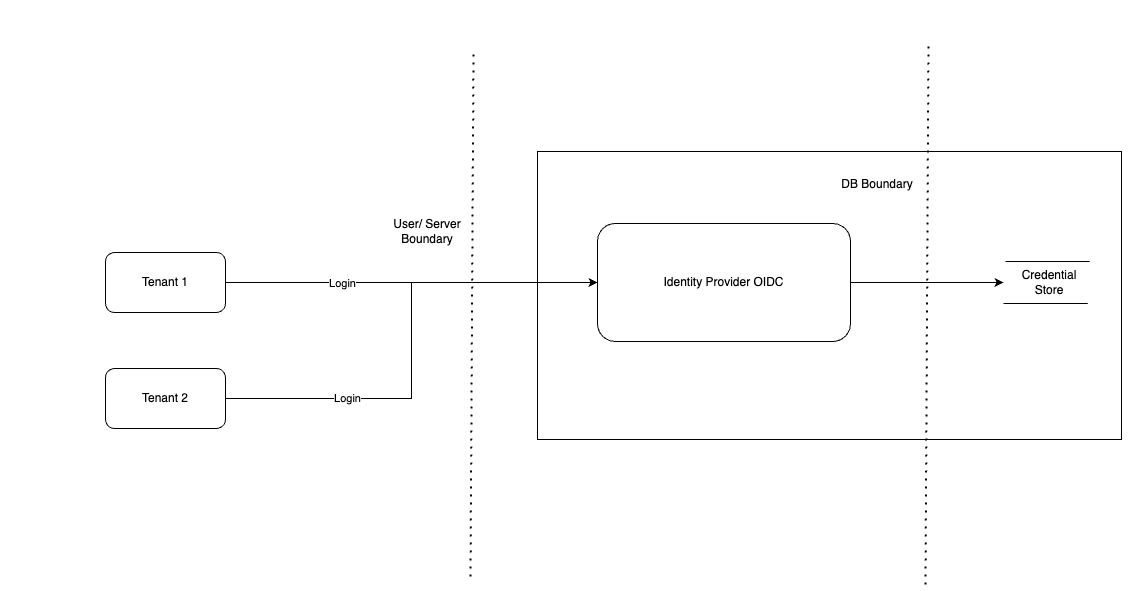
\includegraphics[width=\textwidth, height=320px]{pics/DFD_APP.png}
\end{figure}


\label{subsec:stride}
\subsection*{1. Spoofing}
\begin{itemize}
    \item \textbf{Threat}: An attacker attempts to impersonate a legitimate user or tenant to gain unauthorised access.
    \item \textbf{Specific Attacks}:
    \begin{itemize}
        \item \textbf{ID Spoofing}: The attacker tries impersonating an End user from another OpenID Provider by using spoofed tokens or changing the token's contents \citep{oidc_attacks}.
        \item \textbf{Credential Stuffing}: Using leaked credentials from other services to gain unauthorised access.
        \item \textbf{Phishing}: Tricking users into providing their credentials through fraudulent login pages. For example, the attackers can manipulate the redirect endpoints to redirect to the malicious URL \citep{open_redirect_oidc_threat}.
        \item \textbf{Man-in-the-Middle Attack (MITM)}: Intercepting the authorization code during the OAuth2 flow.
    \end{itemize}
    \item \textbf{Mitigation}:
    \begin{itemize}
        \item Signed tokens should always be verified at the issuer's end so that a spoofed token cannot bypass the security.
        \item The client should validate the audience and issuer claims to prevent tokens from being used across different services.
        \item Enforce multi-factor authentication (MFA) to prevent credential-based attacks.
        \item PKCE mitigates MITM attacks by tying the authorization code to a unique challenge/response.
        \item Use OAuth2’s \texttt{nonce} and \texttt{state} parameters to protect against replay attacks.
    \end{itemize}
\end{itemize}

\subsection*{2. Tampering}
\begin{itemize}
    \item \textbf{Threat}: Unauthorized modification of data or code during transmission or at rest.
    \item \textbf{Specific Attacks}:
    \begin{itemize}
        \item \textbf{Token Tampering}: This attack targets access, ID, and refresh tokens. Where the attacker manipulates the tokens to add their claims and scopes to allow authorised access \citep{oidc_attacks}.
        \item \textbf{Code Injection}: Injecting malicious code or tokens into the OAuth2 flow.
        \item \textbf{OAuth Token Replay}: Reusing an old token after invalidating or expired.
        \item \textbf{Malicious Endpoint} The discovery endpoints of OIDC, such as the ./wellknown, are tampered with, and malicious endpoints are added to the public endpoint where the attacker can now get sensitive information, as the endpoints are fake \citep{oidc_attacks}.
        \item \textbf{Ransomware}: Unlike just OIDC, cloud technologies, especially public clouds, are susceptible to ransomware attacks. In this attack, the attacker tries to misuse existing vulnerabilities and steal sensitive data or encrypt them, making them unusable \citep{ransomeware}.
    \end{itemize}
    \item \textbf{Mitigation}:
    \begin{itemize}
         \item A key should always sign the tokens like ID tokens containing user information and must be verified each time with the issuer when used.
        \item Use PKCE to prevent authorization code injection by requiring a code challenge.
        \item Sign and validate JWT tokens to ensure integrity and detect tampering.
        \item Implement token expiration and invalidation mechanisms and rotating refresh tokens to reduce token reuse.
        \item Use different tools to detect anomalies in the system and prevent malware such as ransomware from propagating deep into different services into the cloud \citep{ransomeware}.
        \item Perform network segregation and build zero privilege systems to allow only the required actors to access the services and no more \citep{zero_trust}. 
    \end{itemize}
\end{itemize}

\subsection*{3. Repudiation}
\begin{itemize}
    \item \textbf{Threat}: Users or tenants could deny performing certain actions, making it difficult to establish accountability.
    \item \textbf{Specific Attacks}:
    \begin{itemize}
        \item \textbf{Action Denial}: A malicious tenant denies having issued a token or performed an action within the application that could deny sending or receiving messages in a digital transaction \citep{repudiation}.
        \item \textbf{Tenant Switching}: Similarly, in a multi-tenant environment, a user might gain access to another tenant’s data and deny the action.
    \end{itemize}
    \item \textbf{Mitigation}:
    \begin{itemize}
        \item Use signed access tokens (JWT) with non-repudiation attributes.
        \item Log every critical action and tenant interaction, including token issuance and API calls, with cryptographically signed entries.
        \item Use immutable logs with encryption.
    \end{itemize}
\end{itemize}

\subsection*{4. Information Disclosure}
\begin{itemize}
    \item \textbf{Threat}: Sensitive data such as access tokens, personal data, or tenant-specific information is exposed.
    \item \textbf{Specific Attacks}:
    \begin{itemize}
        \item \textbf{Cross-Tenant Data Leakage}: Improper multi-tenant isolation could make one tenant’s data accessible to another.
        \item \textbf{Token Exposure}: OAuth2 tokens might be leaked through insecure communication.
        \item \textbf{Cloud Misconfigurations}: Misconfigured database leading to data exposure.
    \end{itemize}
    \item \textbf{Mitigation}:
    \begin{itemize}
        \item Implement strong tenant isolation at the application and database levels, ensuring no cross-tenant data leakage.
        \item Use end-to-end encryption and enforce HTTPS for all communications.
        \item Conduct regular security audits to identify cloud misconfigurations.
        \item Manage whitelisted redirect URIs and limit callback URLs to trusted domains.
        \item Use automated tools to scan for and fix misconfigurations like OWASP Zap \citep{owasp_zap}.
    \end{itemize}
\end{itemize}

\subsection*{5. Denial of Service (DoS)}
\begin{itemize}
    \item \textbf{Threat}: An attacker may overwhelm the service, making it unavailable for legitimate users and tenants.
    \item \textbf{Specific Attacks}:
    \begin{itemize}
        \item \textbf{Token Bombing}: Repeatedly requesting tokens using valid credentials to overload the authorization server.
        \item \textbf{API Rate Limiting Attack}: Flooding API endpoints with excessive requests, leading to resource exhaustion.
        \item \textbf{Resource Starvation}: Exploiting vulnerabilities to consume cloud resources, like CPU or memory, disrupting multi-tenant services.
    \end{itemize}
    \item \textbf{Mitigation}:
    \begin{itemize}
        \item Implement API rate limiting and token request throttling to prevent a token bombing.
        \item Use distributed denial of service (DDoS) protection services, such as AWS Shield \citep{aws_shield}.
        \item Ensure each tenant has isolated resource pools to avoid one tenant's traffic affecting others.
        \item Implement service quotas for resource consumption per tenant.
    \end{itemize}
\end{itemize}

\subsection*{6. Elevation of Privilege}
\begin{itemize}
    \item \textbf{Threat}: An attacker could gain higher privileges than authorised, allowing access to sensitive data or functionality.
    \item \textbf{Specific Attacks}:
    \begin{itemize}
        \item \textbf{PKCE Downgrade Attack}: The attacker can remove \texttt{code\_challenge} from the request if the authentication server does not validate the \texttt{code\_verifier}, the token will be issued, allowing unauthorised access \citep{oidc_attacks}.
        \item \textbf{Insecure Multi-Tenant Access Control}: A user accessing other tenants' resources through misconfigured roles or policies.
    \end{itemize}
    \item \textbf{Mitigation}:
    \begin{itemize}
        \item The \texttt{code\_verifier} must be verified at the authentication server and the \texttt{code\_challenge} should be bound the the authorisation code \citep{oidc_attacks}.
        \item Regularly audit role assignments, permissions, and token scopes to detect misconfigurations.
        \item Implement tenant-aware access control to ensure that users can only interact with resources belonging to their tenant.
    \end{itemize}
\end{itemize}


\section{Risk Assessment}
Risk assessment is integral to keeping a system safe as it helps identify, analyse and evaluate the potential risks that could negatively impact an organization. Cyber breaches have an enormous impact on an organizations value and reputation; for example, in 2024 \citep{ibm} estimated the average cost of a cyberattack on a company in the US is about 4.88M USD. In addition, such data breaches also could cost firms penalties due to non-compliance, especially in the EU. Organisations face hefty fines of up to 10 Million Euros or 2\% of their worldwide revenue under GDPR Article 83 \citep{gdpr_fine}. Therefore, carrying out a risk assessment helps understand the impact of these risks and determine how to manage and address the potential issues before they occur. 

In the cybersecurity space, there are several well-known risk assessment frameworks like Factor Analysis of Information Risk [FAIR], Operationally Critical Threat Asset and Vulnerability Evaluation [OCTAVE], NIST Cybersecurity Framework, and ISO/IEC 27001 \citep{cybersec_risk_frameworks}. Each of these frameworks has its strengths and weaknesses; for example, FAIR considers the frequency of attacks and provides valuable information regarding financial losses \citep{fair_bn}, and OCTAVE and NIST also have their advantages. However, the framework ISO/IEC 27001:2022 is chosen for this project, as this standard focuses exclusively on information security risk management and offers guidance on identifying, accessing, and information systems \citep{iso}. Choosing ISO 27001:2022 provides a significant advantage in its alignment with the ISO/IEC 27000 family, a recognized standard for establishing an Information Security Management System (ISMS). In addition to its compatibility with ISO 27001:2013, this assessment method provides flexibility in adapting to different industries and their sizes. \cite{iso_2700:2022} also states that ISO/IEC 27001:2022 slightly improved to ISO/IEC 27001:2013, consisting of additional protection to cloud computing services, which is also being analysed in this assessment. Following this framework, the following sections will define the scope, methodology, limitations, analysis, and non-compliance risks following local laws like GDPR. 


\subsection{Scope}
The first step in this risk assessment process is to define the scope of the ISMS, as it plays a crucial role in identifying, analyzing, and evaluating the risk effectively. Using the scopes, one can limit the analysis to a particular subject and focus on the priorities. The scope is constrained to a small prototype implementing a multi-tenant authentication application using PKCE flow in a Cloud application, which resembles a small business. The IT assets are listed in Table \ref{table:threat_model_assets}, and the physical usage of this application is located in the European Union, meaning the regulatory measures that need to be followed are based in this region, especially GDPR. The key elements that are part of the scope are as follows:
\begin{itemize}
    \item Cloud Security
    \item Multi-tenancy Issues
    \item PKCE Implementation Issues
    \item Data Security and Privacy
    \item Regulatory and Compliance Requirements
    \item Identity and Access Management (IAM)
\end{itemize}

\subsection{Methodology}
One of the benefits of using risk assessment from the ISO/IEC 27000 group is that it does not prescribe a specific methodology for quantitative or qualitative analysis. In contrast to FAIR, which is a quantitative method, qualitative, quantitative, or a mix of both can be applied here. 

The assessment of this project is based on subjective judgment or qualitative analysis rather than quantitative analysis due to the complexity and nature of the risks. For instance, risks identified during threat modelling, such as data isolation, cloud misconfiguration, and shared resource vulnerabilities, are difficult to quantify because they involve unknown factors. Using subjective analysis simplifies the decision-making process and is faster to conduct. To assess the risks meaningfully, we use the Common Attack Pattern Enumeration and Classification (CAPEC) as a reference. CAPEC provides a comprehensive database for the technical exploits used by adversaries and focuses on application security. CAPEC categorizes the general likelihood and severity into five levels, ranging from very low to very high. These levels are then converted to a number from 1-5 for each to determine the risk level for a specific threat (CAPEC). (See Figure \ref{fig:ris_assessment_method}). 

\begin{figure}[h!]
\centering
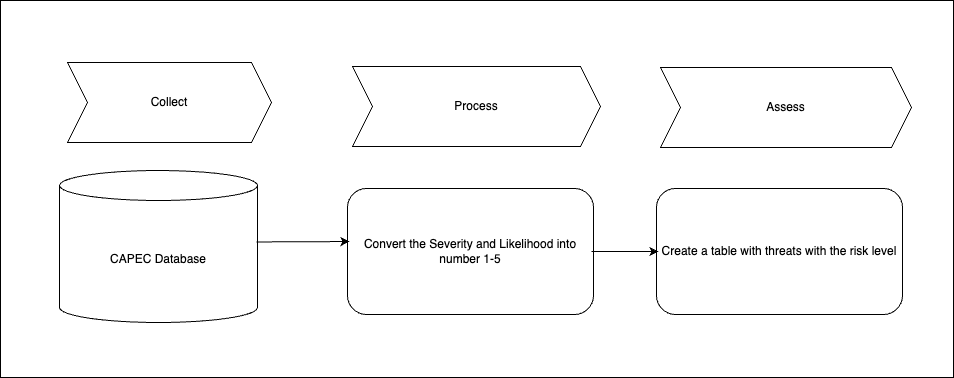
\includegraphics[width=\textwidth]{pics/risk_assessment_method.png}
\caption{Risk Assessment Methodology}\label{fig:ris_assessment_method}
\end{figure}

\newpage
\textbf{Definitions}:
    \begin{itemize}
        \item  \textbf{Likelihood (1-5)}: Likelihood of the attack happening based on the current environment, known vulnerabilities, and ease of exploitation.          \begin{itemize}
            \item \textbf{1}: Very unlikely
            \item \textbf{5}: Very likely
         \end{itemize}
        \item \textbf{Impact (1-5)}: Impact of the attack on the system, focusing on data breaches, financial loss, service downtime, and customer trust.
         \begin{itemize}
            \item \textbf{1}: Very Low
            \item \textbf{5}: Very High
         \end{itemize}
         
       \item  \textbf{Risk Level (1-25)}: Calculated as Likelihood × Impact. High values indicate higher overall risk. 
       \begin{itemize}
           \item \textbf{1-5}: Very Low Risk = Requires minimal attention.
           \item \textbf{5-10}: Low Risk = Requires minimal attention.
           \item \textbf{10-15}: Medium Risk = Needs monitoring and potentially preventive measures.
           \item \textbf{15-20}: High Risk = Immediate action required to mitigate the risk.
           \item \textbf{20-25}: Very High Risk = Immediate action required to mitigate the risk.

       \end{itemize}
    \end{itemize}

    
\subsection{Limitations}  
Although ISO/IEC 20071:2022 is an internationally recognized standard for risk assessment, the framework and scope of this project have some limitations. The limitations of using this methodology for this project are listed below:

\begin{itemize}
    \item Given the timeframe of this project and the limited resources, not all aspects of this framework can be implemented and documented. Instead, only the scope, methodology, and risk assessment.
    \item It is very resource intensive, and the assessment result is based on a specialist doing the analysis, which could lead to subjective arguments.
    \item The project's scope is narrow, mainly focusing on the technical risks of this implementation. This could leave some specific systems not being covered. For example, the amount of financial loss that would occur with different risks is not covered.
    \item The data used from CAPEC to derive the likelihood and impact is a generic value and can differ from the actual case, which could cause some deviation from the analysis.
    \item Some attacks are not listed in the CAPEC database, which then is assessed subjectively according to their complexity and impact. 
\end{itemize}

\subsection{Analysis}
 The analysis section is one of the most critical components, forming the backbone of the research findings. It consists of data on the threats that affect the OpenID Connect application in a cloud environment. The data for the analysis are gathered using various methods, e.g., research papers, journals, and theses. To answer the research question (See \ref{sec:objectives}) mentioned in Chapter 1, the different technical threats and risks that occur due to non-compliance to regulations are analysed. As the methodology mentions, the collected threats are compared against the CAPEC database and are qualitatively assessed. Table \ref{table:risk_assessment} shows the threats analysed, and the risk level is ordered from highest to lowest. 

\definecolor{ForestGreen}{rgb}{0.13, 0.55, 0.13}

\begin{longtable}{|p{4cm}|p{2cm}|p{2cm}|p{2cm}|p{3cm}|}
\caption{Table: Risk Assessment}
\label{table:risk_assessment}
\hline
\rowcolor{grey!15}
\textbf{Threat} & \textbf{Likelihood (1-5)} & \textbf{Impact (1-5)} & \textbf{Risk Level (1-25)} & \textbf{CAPEC ID}\\
\hline
\endfirsthead

\hline
\rowcolor{grey!15}
\textbf{Threat} & \textbf{Likelihood (1-5)} & \textbf{Impact (1-5)} & \textbf{Risk Level (1-25)} & \textbf{CAPEC ID}\\
\hline
\endhead

\hline
\endfoot

\hline
\endlastfoot
Cloud Misconfigurations & 4 & 5 & \cellcolor{red!90} 20 & - \\
\hline
Phishing & 4 & 5 & \cellcolor{red!90} 20 & CAPEC-98  \\
\hline
Man-in-the-Middle (MITM) & 4 & 5 & \cellcolor{red!90} 20 &  CAPEC-94\\
\hline
Credential Stuffing & 4 & 4 & \cellcolor{red!60} 16 & CAPEC-600 \\
\hline
Code Injection (XSS, SQLi) & 4 & 4 & \cellcolor{red!60} 16 & CAPEC-242 \\
\hline
Token Tampering & 4 & 3 &  \cellcolor{yellow!90} 12 &CAPEC-39 \\
\hline
Ransomware & 3 & 4 &  \cellcolor{yellow!90} 12 & CAPEC-549 \\
\hline
Insecure Multi-Tenant Access Control & 3 & 4 &  \cellcolor{yellow!90} 12 & - \\
\hline
Action Denial (Denial of Service) & 4 & 3 &  \cellcolor{yellow!90} 12 & CAPEC-125\\
\hline
ID Spoofing & 3 & 3 &  \cellcolor{green!20} 9 & CAPEC-151\\
\hline

PKCE Downgrade Attack & 2 & 4 & \cellcolor{green!20} 8 & -\\
\hline
Cross-tenant data Leakage & 1 & 4 &  \cellcolor{ForestGreen} 4 & CAPEC-546 \\
\hline

\end{longtable}
 In total, 12 threats were analysed and ranked according to their risk level. Figure \ref{fig:Risk Level Counts} depicts a bar chart showing the risk level vs the count. This analysis identified three very high, two high, four moderate, two low and one very low risk. The mitigations for these threats have already been mentioned in Sub-Section \ref{subsec:stride}; however, this section highlights the level of risk each threat poses to an organization. The high and high risks must be mitigated before the application is published. 

\begin{figure}[h!]
\centering
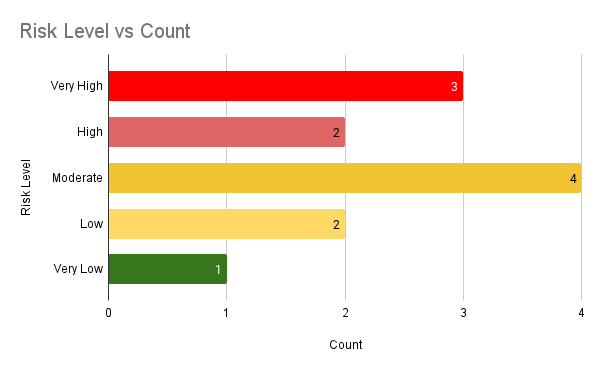
\includegraphics[width=\textwidth]{pics/risk_level_vs_count.png}
\caption{Risk Assessment Methodology}\label{fig:Risk Level Counts}
\end{figure}

\subsection{Non-Compliance Risk}
Non-compliance is a failure to adhere to established laws, regulations, and standards, especially in today's digital age, where vast amounts of sensitive data are also called personally identifiable information (PII). Such personal data are stored, processed, and transferred among different firms. Therefore, protecting private data is a significant priority; hence, various laws and rules bind companies and organisations to protect sensitive data. One of the most stringent data protection frameworks globally is the GDPR act, concerned with data processing of EU residents \citep{gdpr_stringent}. 

Operating an OpenID Connect application in the cloud carries a high risk if it does not comply with GDPR laws. OpenID Connect involves handling personal data, such as user information, so ensuring compliance with GDPR is crucial when working with such an application. To avoid the risk of non-compliance with GDPR, potential financial loss, and damage to reputation, specific key mitigations need to be implemented before publishing the applications. The following are the key provisions from \citep{gdpr_law} that present potential risks according to the GDPR law:


\begin{itemize}
    \item \textbf{Article 6 GDPR}: There should be a lawful basis for processing personal data to fulfil a contractual obligation for the data controller. Organizations must document the lawful basis for processing personal data and ensure transparency in informing users about why their data is being processed. In addition, this article also states the requirement of consent with concise text without vague legal jargon and the functionality to withdraw consent.
    
    \item \textbf{Articles 15-22 GDPR}: Data subject rights: proper access, rectification, erasure, and portability. These rights should be able to exercised by the users. 

    \item \textbf{Article 32 GDPR }: Appropriate Security measures must be taken to protect sensitive data, such as encrypting data, maintaining access control lists, regular audits, and security checks. Failure to implement these measures can result in security breaches, leading to unauthorized access to personal data and violations of GDPR’s security requirements.
    
    
    \item \textbf{Chapter V GDPR }: Cloud based applications often operate across borders. This makes it more important to consider where sensitive data such as PII are stored. GDPR imposes strict rules on transferring personal data to countries outside the European Economic Area (EEA) unless those countries have been deemed to provide adequate data protection. This chapter of GDPR stipulates that providers that are also located outside the EEA must be compliant with GDPR rules. As popular cloud providers such as AWS, Google, and Microsoft operate outside the EEA, this law plays a big role with cloud providers.  
.
\end{itemize}

\section{Conclusion}

Conducting a thorough risk assessment for an OpenID Connect application deployed in the cloud is crucial to identify potential security vulnerabilities and ensure GDPR compliance. OIDC applications handle sensitive personal data during user authentication and authorization, making them susceptible to threats such as cloud misconfigurations, phishing, man-in-the-middle (MITM) attacks, token tampering, and cross-tenant data leakage. These threats can significantly impact personal data's confidentiality, integrity, and availability. 

Therefore, using the threat modelling results, we identified the threats and their mitigations, and the qualitative risk analysis helped us rank these threats according to their risk level. By arranging the threats according to their perceived risk, they can be prioritized to be more efficient. In addition to the threats, the consequence of not following GDPR will also cost the organisation a lot of money, which is a high risk. Based on these results, the high-risk threats have to be applied with the GDPR measures to ensure regulatory adherence. 








